%-------------------------------Aspect Delta---------------------------------
\section{Aspect Delta}

Aspect $\delta$ is a dimensionless number defined as the smallest ratio of the
height of a vertex above its opposing triangle (see Figure~\ref{f:tet-height}) to
the square root of the area the triangle across all vertices of the tetrahedron. 
\begin{figure}[bhp]
  \centering
  \includegraphics[width=1.5in]{tet-height}
  \caption{
    An illustration of the height $h_3$ of vertex 3.%
                                                          \label{f:tet-height}}
\end{figure}
In general, take $(i,j,k,\ell)$ to be a permutation of $\{0,1,2,3\}$
(i.e., $(i,j,k,\ell)\in\Sf$) and $\normvec{ L_{ab}}$ to be the length of the edge
connecting vertices $a$ and $b$.
Then aspect ratio $\delta$ may be written
\[
  q = \min_i\left\{C\frac{h_i}{\sqrt{A_{jk\ell}}}\right\}
\]
where $A_{jk\ell}$ is the area of the triangle opposite vertex $i$ and
$C = \frac{\sqrt[4]{108}}{4}\approx 0.805927$ chosen so that an equilateral tetrahedron has $q = 1$.
PATRAN~\cite{patran:03} also speaks of a ``normalized'' aspect ratio defined as
\[
  q_{alt} = 1 - q = 1 - \min_i\left\{C\frac{h_i}{\sqrt{A_{jk\ell}}}\right\}
\]
which is 0 for an equilateral tetrahedron.

\tetmetrictable{aspect $\delta$}%
{$1$}%                                                Dimension
{$[0.1,DBL\_MAX]$}%                                   Acceptable range
{$(0,DBL\_MAX]$}%                                     Normal range
{$[0,DBL\_MAX]$}%                                     Full range
{$1$}%                                                Equilateral tet
{\cite{patran:03}}%                                   Citation
{\nsup}%                                              Verdict function name


